\section{GİRİŞ}
Günümüzde teknolojik çalışmaların karmaşıklığı ve iş yükünün artmasıyla birlikte, verimli ve ölçeklenebilir bir altyapı tasarımı büyük önem taşımaktadır. Bu nedenle, Web Tabanlı Konteyner Orkestrasyon Sistemi, çalışma olarak ideal bir çözüm değerlendirilmiştir.

Konteyner kavramı, ilk olarak 1979 yılında ortaya atılmış ve o tarihten itibaren gelişimini sürdürmüştür. Bu süreçte Unix V7 ile ilk kez kullanılmıştır. FreeBSD Jails, Linux VServer, Oracle Solaris Containers, Open VZ, Process Containers (Google), LXC, Warden ve Lmctfy gibi gelişim süreçlerinden geçerek günümüze kadar gelmiştir.

Konteyner teknolojisinin daha yaygın hale gelmesi, 2000'li yılların başında FreeBSD Jail ile gerçekleşmiştir. Ardından Jacques Gélinas'in VServer çalışması ile Linux ortamına dahil olmuştur. Bu temel altyapının oluşturulmasının ardından, günümüz Linux konteynerlerinin yapısı şekillenmeye başlamıştır.

Ancak, konteyner teknolojisi bu gelişmelere rağmen hala genel kullanım için yaygın değildi. 2008 yılında Docker, bu alanda devrim niteliğinde bir adım atmıştır. Google gibi büyük bilgi teknolojileri şirketlerinin kullandığı bu sistem, son kullanıcıların da hizmetine sunulmuş ve konteyner teknolojisinin hızla gelişmesine yol açmıştır. Docker, kendi adını taşıyan konteyner teknolojisiyle (dotCloud aracılığıyla) kullanıcıları tanıştırmıştır.\cite{container}

Bu çalışma için Docker'ın kullanılması uygun görülmüştür. Bunun temel nedenleri arasında hafiflik, taşınabilirlik, ölçeklenebilirlik, kolay dağıtım ve yönetim, izolasyon ve güvenlik avantajları bulunmaktadır. Bu tasarım yaklaşımı, çalışmanın gereksinimlerini etkin bir şekilde karşılamak ve iş yükünü yönetmek için ideal bir çözüm sunmaktadır.

Bu çalışmanın amacı, kullanıcıların konteyner teknolojileriyle etkileşimde bulunabilmesini sağlayan bir web arayüzü sunmak ve aynı zamanda konteynerlerin paralel bir şekilde çalışmasını sağlamaktır. Bu arayüz sayesinde kullanıcılar konteyner oluşturabilir, bu konteynerleri paralel olarak çalıştırabilir ve işlemlerin çıktılarını görüntüleyebilirler.

Çalışma sonucunda, konteyner kullanımını kolaylaştırmak amacıyla konteyner oluşturma, çalıştırma, paralel işlemler yapma ve sonuçları görme işlemleri başarıyla gerçekleştirilmiştir. Bu sayede kullanıcılar, konteyner teknolojilerini daha etkili bir şekilde kullanabilir ve işlemlerini daha verimli bir şekilde yönetebilirler.

Web arayüzü sayesinde kullanıcılar, konteynerlerin oluşturulması için gerekli parametreleri belirleyebilir, bu konteynerleri istedikleri işlemleri gerçekleştirmek için kullanabilir ve işlemlerin sonuçlarını  takip edebilirler. Ayrıca, paralel işlemler sayesinde birden fazla konteyner aynı anda çalıştırılarak işlem hızı artırılabilir ve daha fazla veri işlenebilir.

Bu çalışma, konteyner teknolojilerinin kullanımını daha erişilebilir hale getirerek, kullanıcıların konteynerlerle etkileşimde bulunmasını ve paralel işlemler yapmasını sağlamaktadır. Bu da hem geliştiricilerin hem de sistem yöneticilerinin işlerini kolaylaştırabilir ve verimliliklerini artırabilir. Şekil 'de bu projenin çalışma yapısı gösterilmiştir.
\begin{figure}[H]
	\centering
	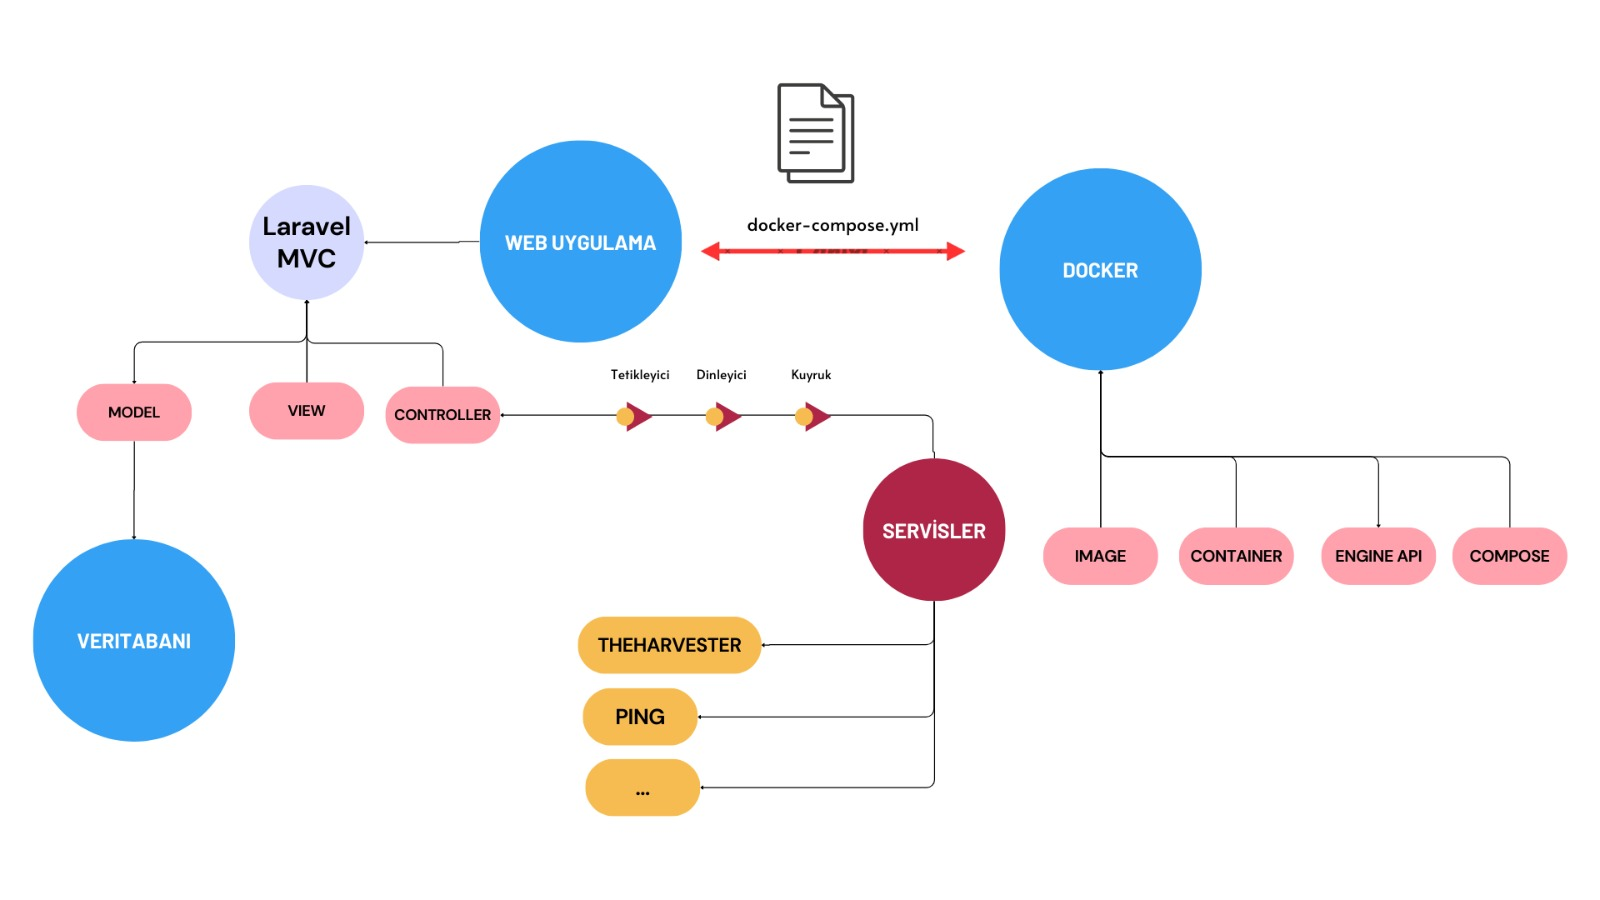
\includegraphics[width=1\linewidth]{images/project.jpeg}
	\caption{Proje Çalışma Yapısı}
	\label{fig:task_diagram}
\end{figure}

Çalışmayla ilgili yapılan araştırmanın bir bölümü olan Literatür Taraması, sonraki bölümde detaylı olarak açıklanmıştır.
\section{LİTERATÜR TARAMASI}
Konteynerizasyon konusunda akademik çalışmalar 2008 yıllarında başlamış, 2013 yıllarından sonra yoğunlaşmıştır. Bu çalışmada konuya yakın olan daha önce yapılan çalışmalar aşağıda özetlenmiştir.

"An Overview of Containerization Technology: Advantages, Challenges, and Future Directions" adlı çalışmada, yazarlar containerization teknolojisinin genel bir bakışını, avantajlarını, zorluklarını ve gelecekteki yönelimlerini ele almaktadır. Makale, containerization teknolojisinin nasıl çalıştığına, sanallaştırma teknolojileriyle karşılaştırılmasına ve çeşitli kullanım senaryolarına odaklanmaktadır \cite{Smith_Emily}.

"Docker for Multi-containers Web Application" başlıklı makalede, Sharma, Saxena ve Singh, çoklu konteyner web uygulamaları için Docker teknolojisini ele almaktadır. Makale, 2020 2. Uluslararası Sanayi Uygulamaları İçin Yenilikçi Mekanizmalar konferansında sunulmuştur. Yazarlar, Docker teknolojisinin kullanımıyla çoklu konteyner web uygulamalarının nasıl hazırlanacağını ve dağıtılacağını ele almaktadırlar. Makalede, Docker'in kullanımının avantajları ve web uygulamaları için uygunluğu da tartışılmaktadır \cite{sharma2020docker}.

"Containerization: A Systematic Literature Review" başlıklı çalışma, containerization teknolojisi hakkında sistematik bir literatür taraması sunmaktadır. Yazarlar, containerization teknolojisinin farklı yönlerini, kullanım alanlarını, avantajlarını ve zorluklarını analiz etmektedirler. Ayrıca, çalışmada gelecekteki araştırma yönelimleri ve containerization teknolojisinin geliştirilmesi için öneriler de sunulmaktadır \cite{Brown_Jennifer}.

"Mastering Docker" adlı kitap, Docker teknolojisi hakkında kapsamlı bir kılavuz sunmaktadır. Okuyucular, Docker'ın nasıl kullanılacağı, konteynerlerin nasıl tasarlanacağı, dağıtılacağı ve yönetileceği hakkında bilgi edinebilirler. Kitap, uygulama geliştirme ve dağıtım süreçlerinde Docker'ın nasıl kullanılabileceği konusunda pratik bilgiler sunmaktadır. Sonuç olarak, "Mastering Docker" kitabı, Docker teknolojisi hakkında kapsamlı bir kılavuz sunarak, okuyucuların konteynerleştirme ve DevOps becerilerini geliştirmelerine yardımcı olmayı amaçlamaktadır \cite{mckendrick2020mastering}.

"On Enhancing the Orchestration of Multi-container Docker Applications" başlıklı makale, Docker teknolojisi ile oluşturulmuş çoklu konteynerli uygulamaların orkestrasyonunu geliştirmek için Docker Compose ile bir alternatif yaklaşım sunmaktadır. Bu çalışma, yazılım geliştiricilere ve sistem yöneticilerine fayda sağlamayı amaçlamaktadır \cite{brogi2020enhancing}.

"Docker Compose'un Çok Bileşenli Sistemleri Oluşturmak İçin Kullanımının İncelenmesi" başlıklı makale, Docker Compose'un kullanımının çoğu zaman çok bileşenli sistemlerin oluşturulması için yararlı olduğunu inceliyor. Bununla birlikte, Docker Compose dosyalarının kullanımı konusunda belirli zorluklar da bulunmaktadır. Örneğin, Docker Compose dosyalarının oluşturulması ve yönetilmesi karmaşık olabilir ve Docker Compose dosyalarının sürdürülebilirliği sorunları ortaya çıkabilir \cite{ibrahim2021study}.

Bu literatür taraması, Docker teknolojisi ve konteynerleştirme üzerine yapılmış bazı çalışmaları özetlemektedir. Bu çalışmalar, Docker'ın çoklu konteyner uygulamaları, orkestrasyon yöntemleri ve kullanım zorlukları gibi farklı yönlerini ele almaktadır. Bu bilgiler, bu çalışmada kullanılan teknolojik seçimlerin nedenleri ve özellikleri hakkında bilgi vermektedir.